\chapter{Bucles y recursividad}
   \label{Bucles}
   \index{Bucles}

\textsc{XLogo} tiene cinco primitivas que permiten la construcci\'on
de bucles: \texttt{repite},\index{repite@\texttt{repite}}
\texttt{repitepara},\index{repitepara@\texttt{repitepara}}
\texttt{mientras},\index{mientras@\texttt{mientras}}
\texttt{paracada}\index{paracada@\texttt{paracada}} y
\texttt{repitesiempre}.\index{repitesiempre@\texttt{repitesiempre}}

\section{Bucle con \texttt{repite}}
   \label{Bucle-con-repite}

Esta es la sintaxis para \texttt{repite}:
\begin{verbatim}
   repite n [ lista_de_comandos ] \end{verbatim}
\texttt{n} es un n\'umero entero y \texttt{lista\_de\_commandos} es
una lista que contiene los comandos a ejecutarse. El int\'erprete
\textsc{XLogo} ejecutar\'a la secuencia de comandos de la lista
\texttt{n} veces. Esto evita copiar los mismos comandos repetidas
veces. \\ 

\noindent \textbf{Ejemplos}:

\texttt{repite 4 [avanza 100 giraderecha 90]}\verb+    +
     \texttt{\# un cuadrado de lado 100} \\

\texttt{repite 6 [avanza 100 giraderecha 60]}\verb+    +
     \texttt{\# un hex\'agono de lado 100} \\

\texttt{repite 360 [avanza 2 giraderecha 1]}\verb+     +
     \texttt{\# abreviando, casi un c\'irculo} \\*[0.3cm]

\noindent Observa que con el bucle \texttt{repite}, se define una variable interna
\texttt{contador} \index{contador@\texttt{contador}} o
\texttt{cuentarepite}, \index{cuentarepite@\texttt{cuentarepite}}
que determina el n\'umero de la iteraci\'on en curso (la primera iteraci\'on
est\'a numerada con el 1)

\begin{verbatim}
  repite 3 [escribe cuentarepite]
  repite 3 [escribe contador] \end{verbatim}
   proporcionan ambas
   \begin{verbatim}
   1
   2
   3 \end{verbatim}

\section{Bucle con \texttt{repitepara}}
   \label{Bucle-con-repitepara}

\texttt{repitepara} hace el papel de los bucles \texttt{for} en otros
lenguajes de programaci\'on. Consiste en asignar a una variable un n\'umero
determinado de valores comprendidos en un intervalo y con un incremento
(paso) dados. Su sintaxis es:
\begin{verbatim}
   repitepara [ lista1 ] [ lista2 ] \end{verbatim}
La \texttt{lista1} contiene tres par\'ametros: el nombre de la variable
y los l\'imites inferior y superior del intervalo asignado a la variable.
Puede a\~nadirse un cuarto argumento, que determinar\'ia el incremento
(el paso que tendr\'ia la variable); si se omite, se usar\'a 1 por defecto.
\begin{quote}
   \noindent \textbf{Ejemplo 1}:
   \begin{verbatim}
  repitepara [i 1 4] [escribe :i*2] \end{verbatim}
   proporciona
   \begin{verbatim}
   2
   4
   6
   8 \end{verbatim}

   \noindent \textbf{Ejemplo 2}:
   \begin{verbatim}
  # Este procedimiento hace variar i entre 7 y 2, bajando de 1.5 en 1.5
  # nota el incremento negativo
  repitepara [i 7 2 -1.5]
    [es lista :i potencia :i 2] \end{verbatim}
   proporciona
   \begin{verbatim}
   7 49
   5.5 30.25
   4 16
   2.5 6.25 \end{verbatim}
\end{quote}

\section{Bucle con \texttt{mientras}}
   \label{Bucle-con-mientras}

Esta es la sintaxis para \texttt{mientras}:
\begin{verbatim}
   mientras [lista_a_evaluar] [ lista_de_comandos ] \end{verbatim}
\texttt{lista\_a\_evaluar} es la lista que contiene un conjunto de
instrucciones que se eval\'uan como booleano (\texttt{cierto} o
\texttt{falso}). \texttt{lista\_de\_comandos} es una lista que contiene
los comandos a ser ejecutados. El int\'erprete \textsc{XLogo} continuar\'a
repitiendo la ejecuci\'on de \texttt{lista\_de\_comandos} todo el tiempo
que \texttt{lista\_a\_evaluar} devuelva cierto. \\

\noindent \textbf{Ejemplos}:

\begin{verbatim}
   mientras ["cierto]
      [giraderecha 1] # La tortuga gira sobre si misma eternamente. 
\end{verbatim}

\noindent \verb+# Este ejemplo deletrea el alfabeto en orden inverso:+

\noindent \texttt{haz \char`\"{}lista1 \char`\"{}abcdefghijklmn\~nopqrstuvwxyz}

\noindent \texttt{mientras [no vac\'io? :lista1]}

\texttt{[escribe \'ultimo :lista1 haz "lista1 menos\'ultimo :lista1]} 

\section{Bucle con \texttt{paracada}}
   \label{Bucle-con-paracada}

La sintacis de \texttt{paracada} es:
\begin{verbatim}
   paracada nombre_variable lista_o_palabra [ lista_de_comandos ] \end{verbatim}
La variable va tomando como valores los elementos de la lista o los caracteres de
la palabra, y las \'ordenes se repiten para cada calor adquirido.

\noindent \textbf{Ejemplos}:

\begin{verbatim}
   paracada "i "XLogo
      [escribe :i] \end{verbatim}
muestra:
\begin{verbatim}
 X
 L
 o
 g
 o
\end{verbatim}

\begin{verbatim}
   paracada "i [a b c]
      [escribe :i] \end{verbatim}
muestra:
\begin{verbatim}
 a
 b
 c
\end{verbatim}

\begin{verbatim}
   haz "suma 0
   paracada "i 12345
      [haz "suma :suma+:i] \end{verbatim}
muestra:
\begin{verbatim}
 15\end{verbatim} (la suma de los d\'igitos de 12345)

\section{Bucle con \texttt{repitesiempre}}
   \label{Bucle-con-repitesiempre}

Aunque un bucle como este es muy peligroso en programaci\'on, ya vimos al explicar
el bucle \texttt{mientras} un ejemplo donde puede simularse un bucle infinito. La
sintaxis es:
\begin{verbatim}
   repitesiempre [ lista_de_comandos ] \end{verbatim}
El ejemplo anterior ser\'ia:
\begin{verbatim}
   repitesiempre [giraderecha 1] # La tortuga gira sobre si misma eternamente. 
\end{verbatim}

De nuevo: \textbf{Mucho cuidado al usar bucles infinitos}

\section{Recursividad}
   \label{Recursividad}

Un procedimiento se llama \textit{recursivo} cuando se llama a s\'i mismo
(es un \textit{subprocedimiento} de s\'i mismo). \index{Recursividad}

Un ejemplo t\'ipico es el c\'alculo del \textbf{factorial}. En lugar de definir

\texttt{n! = n * (n - 1) * \ldots * 3 * 2* 1},

podemos hacer:
 \[ n! = \left\{ \begin{array}{r@{\;\textrm{ si }\;}l}
                  1 & n = 0 \\ n \cdot (n - 1)! & n \neq 0
                \end{array} \right. \qquad \forall \, n \in \mathbbm{N} \]
En \textsc{XLogo}:

\noindent \texttt{para factorial :n\'umero}

\texttt{si :n\'umero = 0}

 \texttt{ [ devuelve 1 ]}

 \texttt{ [ devuelve :n\'umero * factorial (:n\'umero - 1) ]}

\noindent \texttt{fin} \\

\noindent Un segundo ejemplo recursivo es la \textbf{espiral}:

\begin{verbatim}
para espiral :lado
  si :lado > 1250
    [ alto ]
    [ avanza :lado / 500
      giraderecha 1
      espiral :lado + 1 ]
fin \end{verbatim}
\begin{center}
   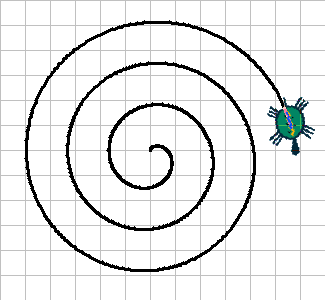
\includegraphics[scale=0.6]{Imagenes/07_Bucles/Espiral.png}
\end{center}
